\documentclass[12pt]{article}
\usepackage[margin=1in]{geometry}
%\usepackage{hyperref}
\usepackage{amsmath}
\usepackage{graphicx}% http://ctan.org/pkg/graphicx
\usepackage{xcolor}
\usepackage{systeme}

%% Make red text
\newcommand{\com}[1]{\textcolor{red}{ #1}}

\linespread{2}

\usepackage[authoryear]{natbib}


\usepackage{tikz}
\tikzset{
  int/.style={circle, draw, fill=blue!20, minimum size=3em},
  init/.style={pin distance=1.2cm,pin edge={loop,thin,black}}
}
\usetikzlibrary{arrows,automata}

\pagenumbering{arabic}

\newcommand{\XX}{\ensuremath{25}} % number of methods

\newcommand{\xxsir}{\ensuremath{11}} % number of SIR methods

\newcommand{\rr}{\ensuremath{\mathcal{R}_0}}

\setlength{\itemsep}{0pt}





\begin{document}




\title{$\XX$ dubious ways of estimating $\rr$}
\author{ Department of Statistics, Carnegie Mellon University}
\date{\today}
\maketitle

%\tableofcontents

\section{Introduction}\label{sec:intro}
What has been called ``arguably the most important quantity in the study of epidemics'', $\mathcal{R}_0$, the reproduction number, has been an elusive quantity to estimate for epidemic modelers for nearly a century \citep{Heesterbeek2002}.  Defined by \citet{anderson1992}, $\rr$ (pronounced $R$-naught) is the ``the average number of secondary infections produced when one infected individual is introduced into a host population where everyone is susceptible.''  $\rr$, in some ways, summarizes an entire outbreak of a disease as this quantity is used whether to assess if a disease will break out and what percentage of the population needs to be vaccinated to avoid such an outbreak.  Despite a clear definition of $\rr$, epidemiologists have struggled to create a \textit{de facto} estimator for $\rr$  \citep{hethcote2000}.  The primary issue in estimating $\rr$ is that the quantity is a \textit{property of the model}, meaning that $\rr$ is dependent not only on the usual noise that comes with statistical modeling but also on a variety of assumptions on how researchers assume a disease is transmitted through a population.

Typically, disease models are a part of the ``SI-framework'' pioneered by Kermack and McKendrick in the 1920s \citep{getz2006}.  Here, S and I are known as compartments where S stands for ``susceptible'' and I for ``infected.''  The issue of estimating $\rr$ stems from how individuals are assumed, either implicitly or explicitly, to move from the S compartment to the I compartment and any other compartments that have been introduced such as immune, recovered, dead, or exposed, for example.  One of the simplest models in the SI framework is the SIR model where R stands for a ``recovered'' state where individuals are no longer susceptible to the disease \citep{Kermack700}.  Even in this simplified framework, there is much dispute on how $\rr$ is to be estimated arising from assumptions on how populations intermix, if any intervention has been put in place, or whether disease parameters are constant over time.

Other issues about estimating $\rr$ include mathematical versus statistical approaches (i.e. solving for $\rr$ versus estimating $\rr$), how to estimate the quantity in the presence of types of available data, and when to estimate $\rr$ in a disease's lifetime.  This depends on the ``time constant'' of the disease.  Some diseases like measles progress rapdily, HIV more slowly, prion diseases glacially so.  For instance, if only weekly incidence counts of a disease are available, then we have different methods of estimating $\rr$ available than when we have more data available such as contact networks or the serial interval of a disease.  Another major issue is that since $\rr$ is so difficult to estimate in the first place, the estimated variance of the estimated $\rr$ has largely been glossed over or  ignored.  This is especially troubling because we are concerned whether $\rr > 1$, which indicates an outbreak of a disease.  A point estimate is simply not enough to determine the truth of this inequality.

In short, $\rr$ is an important parameter in epidemiology that is very difficult to estimate.  This, in turn, makes it difficult to compare $\rr$ across different diseases or even different instances of the same disease.  Many of these challenges with estimating $\rr$ and more are summarized and expanded upon by \cite{li2011}.

We review $\XX$ ways to estimate $\rr$ across a number of model assumptions and in the presence of different sources of data.  The title of this manuscript is in reference to a seminal paper by Moler and Van Loan (1978) (and its subsequent update in 2003) in which they calculate ``Nineteen dubious ways to compute the exponential of a matrix'' \citep{moler2003}.  We not only review the methods of estimating of $\rr$ but also include recommendations on when to use the methods as well as introducing techniques which allow estimation the variance.  We compare these estimates, when applicable, and find that $\rr$ is more robust than what was initially presumed.

The rest of this manuscript is organized as follows.  In Section \ref{sec:overview}, we introduce the methods in four broad groups: the survival function, compartment models, exponential growth models, and agent-based models.    In Section \ref{sec:details}, we give an overview of each of the methods, what assumptions are used, what data is required, and where the method has been used in the past along with ways in which to estimate the variance of the methods, when applicable.  In Section \ref{sec:results}, for a number of different data sets, we give estimates of $\rr$ for the different methods and their variances over a variety of data sets.  Finally, in Section \ref{sec:dis} we discuss our conclusions and recommendations.  In Appendix \ref{sec:term} we include a glossary of terminology used throughout our manuscript.


\section{Overview of $\XX$ Methods to estimate $\rr$}
\label{sec:overview}

In this manuscript, $\XX$ methods were chosen to give a survey of methods for estimating $\rr$.  This is not exhaustive, but these methods were chosen due to historical importance and impact in the field of epidemiology. 

In order to organize the methods for estimating $\rr$, we have chosen four broad classes of estimation methods.  These partitions are meant to be guidelines for distinguishing methods from one another rather than immutable groups.  Many of these methods  fit in  mulltiple of the groups shown.  We have chosen the four groups as application of the survival function and its close relatives, classic compartment models, exponential growth assumptions, and estimation from networks.  We list these point estimate methods below.

\textbf{Point Estimation}
\begin{enumerate}
\item Survival function
  \begin{enumerate}
  \item Survival function (SF)
  \item Direct parameter estimation (DPE)
  \item Von Foerster equations (VFE)

  \end{enumerate}
\item Compartment models 
  \begin{enumerate}
  \item SIR model
    \begin{itemize}
    \item Least squares (SIR LS)
    \item Reparametrized least squares (SIR ReLS)
    \item Linear model approximation (SIR LMA)
    \item Linear model approximation, all time points (SIR LMAT)
    \item Max of data (SIR Max)
    \item Smooth max (SIR SMax)
    \item Incidence-prevalence ratio (SIR IPR)
    \item Smooth incidence-prevalence ratio (SIR SIPR)
    \item Log-linear (SIR LL)
    \item Markov chain estimation (SIR MC)
    \item Sequential Bayes (SIR SB)
    \end{itemize}
  \item SEIR model (SEIR)
  \item MSEIR model (MSEIR)
  \item Amplifier model (AMP)
  \item Next generation model (NGM)
  \end{enumerate}
\item Exponential growth 
  \begin{enumerate}
  \item Exponential growth (EG)
  \item Maximum likelihood of secondary infections (MLSI)
  \item Time dependent reproduction number (TDR)
  \item Initial growth rate and final size  (IGRFS)
  \end{enumerate}
\item Estimation from networks 
  \begin{enumerate}
  \item Contact tracing (CT)
  \item Branching process (BP)
  \item Agent-based models (ABM)
  \end{enumerate}
  \end{enumerate}

  Additionally, we describe  interval estimates for the above methods for estimating $\rr$ in order to better answer the question of whether $\rr > 1$, which implies an outbreak of the disease..  
  
\textbf{Interval Estimation}
\begin{enumerate}
\item Delta method
\item Sensitivity analysis
  \item Posterior distribution
  \end{enumerate}






\section{Details for the $\XX$ methods}
\label{sec:details}
\subsection{Survival function}
\label{sec:direct}

The first set of methods are those of hte survival function, which is closely  tied to the history of $\rr$.  The survival function, which originates from the field of demography in the late 1800s, described how many female offspring a woman would produce \citep{dietz1993estimation}.  In demography, we have
\begin{align*}
\rr = \int_0^\infty p(a) \beta(a) da
\end{align*}
where $p(a)$ denotes the probability of a woman surviving to age $a$ and $\beta(a)$ the rate of an individual of age $a$ giving birth to a  girl.   This interpretation also explains the origins of the name of $\rr$, which was imported to the field of epidemiology by MacDonald and Smith \citep{dietz1993estimation}.  Analogously in epidemiology, $p(a)$ is the age of a disease, and $\beta$ is the transmission rate.

This is the chronologically first, and in many ways, the most direct method to estimate $\rr$.  However, this model also seems to be the most difficult to estimate as both $p(a)$ and $\beta (a)$ are random variables, a distribution and funtion, respectively.  In general, it is also difficult to estimate these parameters before or even during an ongoing disease outbreak.  As such, $\rr$ can only be estimated after an outbreak, which means it cannot be used to determine ongoing prevention strategies.  However, having a post-disease estimation of $\rr$ may be useful for preventing future outbreaks of the disease and aids in comparing the severity of many diseases.  Another advantage of this method is it intuitive and independent of assumptions of how the disease is transmitted from person to person.    We describe four methods attempting to estimate $\rr$ from the survival function:  the survival function alone, direct estimation, and direct parameter estimation.


\subsubsection{Survival Function (SF)}
\label{sec:survival_fxn}
The first method of estimating $\rr$, is not surprisingly, the survival function itself as presented by \cite{Heffernan2005}.  We change the notation from the above survival function to conform to the standards of epidemiology.  

Let $F(a)$ be the probability that a newly infected individual remains infectious for at least time $a$, and let $b(a)$ be the average number of newly infected individuals that an infectious individual will produce per unit time when infected for total time $a$.  Then $\rr$ is derived in Equation (\ref{eq:r0_survivalfxn}),

\begin{align}\label{eq:r0_survivalfxn}
  \rr = \int_0^\infty b(a)F(a)da.
\end{align}

This method presents one of the unique difficulties of estimating $\rr$: that of reconciling generations and time.  $\rr$ tells us about the generations of disease, meaning an infector and tis infected, but not necessarily when the infections occur.  This reconciliation between generations and time is made difficult as the data we have about a disease is often of a temporal nature.  On the other hand, this method is flexible in that this derivation of $\rr$  does not place assumptions on how the disease transmits through a population.  A disadvantage is that data about $F(a)$ and especially $b(a)$ is difficult to collect directly.

Estimating this quantity in Equation \ref{eq:r0_survivalfxn} is hard and, in fact, rarely attempted. It is due to this difficulty that many of rest of the methods for estimating $\rr$ even exist.  



\subsubsection{Direct Parameter Estimation (DPE)}
\label{sec:dpe}

This approach for parameters that are readily available to be estimated, direct parameter estimation, is a `plug and chug' approach as described by \cite{lipsitch2003} and \cite{dietz1993estimation}.  This method has an intuitive derivation, similar to that of the survival function.  We assume that we can estimate $\rr$ if we know how many others an individual comes into contact $(k)$, the probability of transmission given contact $(b)$, and how long the disease lasts within an individual $(D)$.  Then $\rr$ is the product of these parameters, 
\begin{align}\label{eq:dpe}
\rr = kbD.
\end{align}
\cite{lipsitch2003} note that directly estimating $\rr$ in such a way may be difficult due to the available data, as in the previous two methods.  They instead estimate $\rr$ using the mean serial interval, $\omega$, the time from onset of symptoms in an index case to the onset of symptoms in a subsequent case infected by the index patient in addition to the assumption of exponential growth of infected cases, as a proxy for the duration $D$.  Advantages of this method is that it reduces the problem to three parameters that we can conceivably collect data on.  Disadvantages include in the event, that the is estimate may be calculated, uncertainty estimates must be compounded, and to estimate $\rr$ alone, we only use data from the initial outbreak of the disease, so often we have a small sample size, resulting in large confidence sets or credible intervals.


%%%%%%%

\subsubsection{Von Foerster Equations (VFE)}
\label{sec:direct-estim-surv}

A derivation of $\rr$ similar to the survival function comes from the idea of the von Foerster equations, which were used to calculate the number of cells in a ``deme,'' a constrained area.  The function $Y(t, \tau)$ calculated the number of cells at age $\tau$ at time $t$ \citep{trucco1965}.  In epidemiology, $Y$ represents the number of infections instead of cells. Letting $Y(t, \tau)$ be the number of infections at time $t$ of age $\tau$ and assuming no deaths in the population, the von Foerster equation is
\begin{align*}
  \frac{\partial Y(t, \tau)}{\partial t} +   \frac{\partial Y(t, \tau)}{\partial \tau} = 0,
\end{align*}
where $Y(t,\tau)$ is the number of people at time $t$ who were infected time $\tau$ ago.    \cite{fraser2004factors} derived an expression for $\rr$ from the von Foerster equation, the additional equation
\begin{align*}
  Y(t,0) &= \int_0^t \beta( \tau) Y(t, \tau) d \tau,
\end{align*}
and initial conditions $Y(0,0) = Y_0$ and $Y(t, \tau) = 0$ when $t < \tau$.  Then the reproduction number is Equation \ref{eq:vfr0},
\begin{align}\label{eq:vfr0}
\rr &= \int_0^\infty \beta(\tau) d\tau,
\end{align}
 where $\beta (\tau)$ represents the infectiousness at time $\tau$ since the infection.    Again, this model is more mathematical in nature than practical as $\beta (\tau)$ is difficult to estimate.  To estimate $\rr$, \cite{fraser2004factors} make an approximation that $Y(t, \tau) = K(\tau) \exp (rt)$ and further adapt the method to include prevention strategies, but the main parameter to be estimated is $\beta (\tau)$.  Estimating $\beta (\tau)$ has many of the same issues as trying to estimate $b(a)$ in the survival function in that it is difficult to estimate while the disease is ongoing but is also advantageous in that it does not place assumptions on how the disease is transmitted throughout the population.


%%%%%%%%%%%%%%%



\subsection{Compartment Models}
\label{sec:cms}

A large and the most common set of methods used estimate $\rr$ is that of fitting compartment models (CMs) to disease data.  As described in \cite{daley2001epidemic},  CMs model how objects move from one discrete state to another over time.  These models provide a high-level model of how diseases may be spread throughout a population.  Within the CM framework, we make four essential assumptions,
\begin{enumerate}
\item The compartments are discrete and have no overlap.
\item The transition of objects into and out of compartments is described by a set of known equations, possibly dependent on unknown parameters.
\item The populations mix homogeneously
  \item The number of objects in each compartment at time $t=0$ is known
  \end{enumerate}  


Another common assumption for compartment models, is the law of mass action, a property borrowed from chemistry which says that the mass of the product is proportional to the mass of the reactants.  In epidemiology, this means that the proportion of new infections is proportional to the current  number of susceptible and infected \citep{anderson1992}.  Therefore, the flow of objects from one compartment to another may be dependent on the percentage of objects within one or many of the compartments. 

For disease modelling, all CMs fall into the SI-framework, meaning that there is a susceptible population that may become infected.  Thus, we require there be susceptible and infected compartments but also allow additional compartments such as the recovered state, an exposed latent state, and more.  CMs may either work with continuous or discrete time and \cite{getz2006} remark that there is no preference between the two.

In this section, we discuss $\xxsir$ different CM-based methods used to estimate $\rr$.  Different model specifications of CMs yield different mathematical derivations of $\rr$.  That is, for example, an SIR model with non-constant population will yield a different mathematical formula for $\rr$ than the SEIR model (here ``E'' stands for exposed) with non-constant population.  The difference in these two models is that the SEIR model has an extra compartment which in turn effects the estimates of transitions from one compartment to another.  That said, even within the same compartment model framework, we can estimate $\rr$ in a variety of ways using statistical techniques.  In fact, we describe 10 methods to estimate $\rr$, within the SIR framework alone!  Most of these methods are recipes to estimate parameters within the SIR model and may be extended to other CM frameworks such as the SEIR model.  The final method described in this section, the next generation operator (NGM) is a general method to derive $\rr$ from any valid CM.  A particular advantage to CMs compared to survival function methods is that it easier to estimate as data that is typically collected about diseases: namely, incidence counts.  




\subsubsection{SIR Model}
\label{sec:sir-model}

We begin with the most well known CM, the SIR model.   First introduced to epidemiology by  \cite{Kermack700}, the SIR model governs how individuals transition from susceptible, infected, and recovered compartments.  The model is represented graphically in Figure \ref{fig::sir}. 

\begin{figure}[h]
\centering
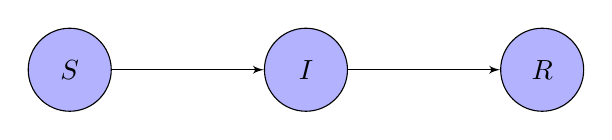
\begin{tikzpicture}[node distance=3cm,auto,>=latex',every node/.append style={align=center}]
    \node [int,  fill = white!70!blue] (a)              {$S$};
    \node [int,  fill = white!70!blue]           (c) [right of=a] {$I$};
    \node [int,  fill = white!70!blue] (e) [right of=c] {$R$};
    \path[->, auto=false] (a) edge node {} (c)
                          (c) edge node {} (e) ;

\end{tikzpicture}
\caption{Depiction of a SIR model.  One can only get the disease once in this model.}\label{fig::sir}
\end{figure}
In this model particular  SIR model, $N$, the number of individuals in constant, as we see no arrows pointing out of the nodes in Figure \ref{fig::sir}. Simple adaptations of the SIR model can include birth and death rates, which may correspondingly change the derivation of $\rr$ (for more information, see Section \ref{sec:ngm}). The parameters  $\beta$ and $\gamma$ have epidemiological meaning.  Here, $\beta$ is the average infection rate and $\gamma$ is the inverse of the average recovery rate.  The transition of individuals from one compartment to another is represented through the ODEs below.  Throughout, we use $X$, $Y$, and $Z$ for stand-ins for the ODEs for $S$, $I$, and $R$, respectively to avoid any confusion with $\rr$.
\begin{align}
\systeme{\frac{dX}{dt} = -\frac{\beta XY}{N}, \frac{dY}{dt} = \frac{\beta XY}{N} - \gamma Y, \frac{dZ}{dt} = \gamma Z}. \label{eq::sir}
\end{align}

In words, susceptible individuals become infected at a rate that is proportional to the proportion of infected individuals multiplied by $\beta$, the infection rate, and the number of susceptible individuals.  Infected individuals recover at a rate of $\gamma$ multiplied by the number of infected individuals.

An epidemic occurs if the rate of change of susceptibles is positive,
\begin{align*}
  \frac{dY}{dt} &> 0 \\
 \frac{\beta S I}{N}  - \gamma I &> 0 ,
\end{align*}

that is,  the rate of new infections is greater than the rate of recovery.  So as long as the number of susceptibles is large, $\frac{S}{N} \approx 1$, then an outbreak will occur if $\rr >1$,
\begin{align}\label{eq:deriv_sir}
  \rr = \frac{\beta}{\gamma} > 1.
  \end{align}
Ideally, we have access data of the number of susceptibles, infecteds, and recovered individuals at different points over time.  From this we would like to estimate the $\beta$ and $\gamma$ parameters and ultimately $\rr$.

There are numerous ways to estimate the parameters in this model.  We detail 10 of them here.  In every one of these methods, it is assumed that the SIR model is the correct specification.

\subsubsection{Least Squares ($\beta$, $\gamma$) (SIR LS)}\label{least-squares-beta-gamma}
The first approach to estimate $\rr$ in the SIR model is simply to minimize the mean square error for the data collected at each time point.  In particular, we find

\begin{align*}
(\hat{\beta}, \hat{\gamma} )&=\text{argmin}_{\beta, \gamma} \sum_{t} (Y(t)_{obs} - Y(t))^2 
\end{align*}

Then  the estimate for $\rr$ is in Equation \ref{eq:sirls},
\begin{align}\label{eq:sirls}
  \hat{R}_0= \frac{\hat{\beta}}{\hat{\gamma}}.
  \end{align}

We can use gradient descent or another optimizer to find estimates for these parameters.  If we assume $Y= f(t) + \epsilon_t$ with $\epsilon_t \overset{iid}{\sim} N(0, \sigma^2)$ where $f(t) = \int_0^t \frac{dY}{dt} dt$, then this this method is equivalent to finding the maximum likelihood estimator (MLE) of $\beta$ and $\gamma$.  However, we note that the the $\epsilon_t$ are very likely not independent from one another and so valid inference is still an issue in this framework.  Even if it were correct, ratio estimations typically result in large, uninformative confidence intervals.   The advantage is that this is a very straightforward way to estimate $\rr$ from the SIR model.

\subsubsection{Reparametrized Least Squares ($\rr$, $\gamma$) ( SIR ReLS)}\label{reparametrized-least-squares-rux5f0-gamma}

In the previous method, we estimated $\beta$ and $\gamma$ and then estimated $\rr$.  However, it is possible to directly estimate $\rr$ if we reparametrize the ODEs in Equation \eqref{eq::sir} directly with \(\rr\) and \(\gamma\), using the relation $\rr = \frac{\beta}{\gamma}$.

\begin{align*}
  \left \{
  \begin{array}{cl}
    \frac{dX}{dt} &= - \rr \gamma Y \frac{X}{N}\\
    \frac{dY}{dt} &=  \rr \gamma Y \frac{X}{N}  - \gamma Y \\
    \frac{dZ}{dt} &=  - \gamma Y 
  \end{array}
  \right .
  \end{align*}

We find

\begin{align*}
(\hat{R}_0, \hat{\gamma} )&=\text{argmin}_{\rr, \gamma} \sum_{t} (Y(t)_{obs} - Y(t))^2 .
\end{align*}

We use the \(\rr\) directly from the above estimation process, which again be done with gradient descent or another optimization process.  Again, we cannot assume $\rr$ has a normal distribution as the errors are likely correlated.  This method is more advantageous in least squares in finding the distribution of $\rr$ as there is no ratio estimation.



\subsubsection{Linear Model Approximation (SIR LMA)}\label{linear-model-approximation-degree-10}

The SIR model has no known closed form solution and so we are already using approximations using numerical integration, albeit small approximations.  In addition to this, data collected from real diseases are typically very noisy in the first place.  \cite{chang2017} discover that an SIR model may be well approximated by a linear model.  We use this idea here and use the ODEs in Equation \eqref{eq::sir} to relate our estimated linear model to that of $\rr$.

Specifically, we fit a linear polynomial of \(t\) with degree \(K= 10\) model to \(X\)
and \(Y\) using least squares to find the coefficients (\(\hat{x}_k\),
\(\hat{y}_k\)),
\begin{align*}
X(t) &= \sum_{k=0}^K x_k t^k\\
{Y}(t) &= \sum_{k=0}^K y_k t^k
\end{align*}
Then, we estimate the derivatives as
\begin{align*}
\hat{X}^\prime(t) &= \sum_{k=1}^K k \hat{x}_k t^{k-1}\\
\hat{Y}^\prime(t) &= \sum_{k=0}^K k \hat{y}_k t^{k-1}
\end{align*}

Following,  \(\rr\) is derived the ODEs,
\[\rr = \frac{\hat{X}^\prime(0)}{ \hat{X}^\prime(0) + \hat{Y}^\prime(0)} \cdot \frac{N}{X(0)}. \]
Like in the previous cases, we are assuming the true models are

\begin{align*}
X(t) &= \sum_{k=0}^K x_k t^k + \epsilon_t\\
  {Y}(t) &= \sum_{k=0}^K y_k t^k + \epsilon_t,
\end{align*}
with $\epsilon_t \overset{iid}{\sim} N(0, \sigma^2)$.  Here, $K=10$ is rather arbitrary and should be selected using some criterion such as AIC in addition with the knowledge of how many data points are available to the user.  Besides this selection of the degree of polynomials to fit, this model is simple to implement and gives very comparable results to using least squares with the SIR model.  Again, we cannot use this model for inference, as our error assumption is violated.  Another disadvantage is that we are using the first time point $t=0$ to estimate $\rr$.  However, as $t=0$ is the boundary of the support of time values, it is likely be a biased estimate as typically seen in linear regression.

\subsubsection{Linear Model Approximation, All Time Points (SIR LMAT)}\label{linear-model-approximation-all-time-points-degree-10}

The above formulation of a linear model approximation only uses the estimate at time $t=0$ to estimate $\rr$.  We can instead, use all time points available to estimate $\rr$.  We fit a linear polynomial of \(t\) with degree \(K= 10\) model to \(X\)
and \(Y\) as above, with a slight modification in how we calculate
\(\rr\),
\[\rr = \frac{1}{\# \text{ Obs }t}\sum_t \frac{\hat{X}^\prime(t)}{ \hat{X}^\prime(t) + \hat{Y}^\prime(t)} \cdot \frac{N}{X(0)} \]
The intuition is that $\frac{X^\prime}{X^\prime + Y^\prime}$ is constant in $t$, but due to our approximations with the linear model, this is no longer the case.  Here, we average over the different possible values of $\rr(t)$.  An advantage to this approach is that we have a more robust estimate of $\rr$ than just using one time point.  The disadvantages are the same as before.

\subsubsection{Max of Data (SIR Max)}\label{max-of-data}
The number of infections curve in the SIR model has one peak.    We note that \(Y^\prime(t) = \frac{\beta XY}{N} - \gamma Y = 0\) when \(\rr = \frac{\beta}{\gamma} = \frac{N(t)}{X(t)}\). The max
of \(Y\) occurs when \(Y^\prime = 0\) and hence
\[\rr = \frac{N}{X_{obs}(t^*)},\] where
\(t^* = \text{arg max}_{t} Y_{obs}(t)\).   A major disadvantage to this method is that it only uses one sample, making it a terrible a statistic and more of a mathematical quantity.  An advantage is that if for instance, one is running simulations, one can make this quick calculation for $\rr$ instead of having to fit a model each time.

\subsubsection{Smooth Maximum of Data (SIR SMax)}\label{smooth-maximum-of-data}

We use a spline with 4 degrees of freedom to fit both \(X\), and \(Y\).
We then apply the principle as above, except now,
\[\rr = \frac{N}{\hat{X}(t^*)},\] where
\(t^* = \text{arg max}_{t} \hat{Y}(t)\).   This approach is a statistical approximation of the previous method of using the smoothed max to estimate $\rr$ instead of a single point.  In this way, we can utilize all our data.  Another advantage is the flexibility in model choice in that we can use a spline, linear regression, or any other model which gives us predictions for the number infected and number of susceptibles.  However, despite this flexibility in model choice, one must remember that we assumed an underlying SIR model for the derivation of $\rr$.

\subsubsection{Incidence to Prevalence
  Ratio (SIR IPR)}\label{incidence-to-prevalence-ratio}
The incidence to prevalence ratio (IPR), described by \cite{Nishiura2009} is another intuitive method to calculate $\rr$ as it incorporates some of most basic epidemiological quantities, incidence and prevalence.

In terms of data from the SIR model, incidence $J(t) \approx -(X(t+1) - X(t))$, and the IPR$(t) = \frac{J(t)}{Y(t)}$. The \textit{actual} reproduction number, $R_a(t) = \text{IPR}(t)\cdot D$ where $D = 1 /\gamma$ the duration of the infection.  This method assumes that we have some prior knowledge about $\gamma$, the transmission rate.  Thus we use as our estimate,
\begin{align*}
\rr &= R_a(0).
\end{align*}

Here we assume that the time step is small enough to approximate the incidence.  The advantage of this method are that incidence data is generally readily available as is prevalence data for certain diseases such as HIV.  However, as one is required to have prior knowledge about $\gamma$, it may be easier to directly estimate $\rr$ with one of the many other methods described that does not require a prior knowledge about $\gamma$.  Again, we are using only one point to estimate $\rr$.

\subsubsection{Smoothed Incidence to Prevalence Ratio (SIR SIPR)}
We use the same method as above, IPR, but first fit splines with 4 degrees of freedom, $\hat{X}(t)$ and $\hat{Y}(t)$, , to fit to $X_{obs}$ and $Y_{obs}$, respectively.  Then  $J(t) \approx -(\hat{X}(t+1) - \hat{X}(t))$, and the IPR$(t) = \frac{J(t)}{\hat{Y}(t)}$.  Then
\begin{align*}
\rr &= R_a(0).  
\end{align*}
The advantage of this method is that it creates a less noisy estimate than estimating IPR using only one point.  It has the same disadvantages as the regular IPR ratio in that it requires knowledge about $\gamma$.

%%%%%%%%%%%%%%%%%%%%%
\subsubsection{Log-Linear (SIR LL)}
Recently, \cite{harko2014exact} were able to reduce the SIR model, with the following set of ODEs (reparametrized from Equation \eqref{eq::sir})

\begin{align*}
  \left \{ \begin{array}{ll}
             \frac{dX}{dt} &= - b X(t) Y(t) \\
             \frac{dY}{dt} &=  b X(t) Y(t) - \gamma Y\\
             \frac{dZ}{dt} &= \gamma Y,\\
           \end{array}
  \right .
\end{align*}

where $b = \frac{\beta}{N}$, to one differential equation.  Letting
\begin{align*}
  u(t) &= e^{\frac{b}{\gamma}Z} \\
  t - t_0 &= \int_{u_0}^u \frac{d \xi}{\xi (C_1 - \gamma \log \xi + X(0) b \xi)},
\end{align*}
where $C_1 = -\frac{b}{N}$, then

\begin{align}
  X(t) &= X(0) u  = X(0) e^{\frac{b}{\gamma}Z(t)} \nonumber\\
  \log \frac{X(t)}{X(0)} &=  \frac{b}{\gamma}Z(t) =  \frac{\beta}{\gamma N} Z \nonumber\\
  N\log \frac{X(t)}{X(0)} &=  \rr Z(t) \label{eq:harko_lin}
\end{align}

If we add error into Equation (\ref{eq:harko_lin}), then we have

\begin{align}
N  \log \frac{X(t)}{X(0)} &=  \rr Z  + \epsilon_t\label{eq:r0_harko}
\end{align}

If we assume $\epsilon_t \overset{iid}{\sim}N(0, \sigma^2)$, then we can directly estimate $\rr$ via linear regression and least squares.  This method greatly simplifies the computational effort needed to estimate $\rr$ as it does not require any numerical integration.  Another advantage is that unlike using the linear approximation method, the coefficient from this model are directly interpretable.  In words, $\rr$ means that for one more recovery, we expect $N \log \frac{X(t)}{X(0)}$ to increase by $\rr$.  A disadvantage is that again, $\epsilon_t$ are  not likely iid.

\subsubsection{Markov chain estimation (SIR MC)}
A natural approach to epidemic modeling is that of Markov chains (MC), since it is assumed an individual's next state is only dependent on its current state.  Much work has been done over the years in this specific field including asymptotic behavior, continuous time MC, confidence intervals, and more \citep{jacquez1991,gani1995,daley2001epidemic}.  We present one the simpler instantiation of the model, the discrete time case, which traces its origin back to the Reed-Frost model \citep{abbey1952}.

In this framework, the number of susceptibles at the current time, $X_{t+1}$ has a binomial distribution based on the contacts with the current number of infected, $Y_t$ and the current number of susceptibles.  That is $X_{t+1} \sim \text{Binom}(X_t, \alpha^{Y_t}$), where $\alpha$ is the probability of avoiding infection from an infective.  \cite{barbour2004} report that the reproduction number is thus,
\begin{align}\label{eq:r0-mc}
\rr &= \log \left ( \frac{1}{1-\alpha}\right ).
\end{align}

Thus, using regression on susceptible/infection counts will lead to an estimate of $\alpha$ and hence $\rr$.  However, this framework typically allows more than just the reproduction number to be estimated.  Through recursion, one can calculate the probability of having a given number of susceptibles and infected at each time step, and hence the entire distribution may be known.





\subsubsection{Sequential Bayes (SIR SB)}\label{sec:seqbayes}

Described by \cite{bettencourt2008} and summarized in \cite{obadia2012r0}, the sequential Bayes method is a Bayesian approach to an approximation of the classic SIR model.  The approximated SIR model assumes that the incidence at $t+1$, $J(t+1)$ has a Poisson distribution, with $\gamma$ as the  average inverse of the infectious period and $\mathcal{R}$ as the effective reproduction number, which we take here to be $\rr$. In order to estimate $\rr$, we must have some idea about $\gamma$,
\begin{align*}
J(t+1)  \sim Poisson( J(t) \exp \left \{  \gamma (\rr-1)\right \})
\end{align*}
Then, the posterior distribution of $\rr$ given the previous days' incidences is
\begin{align*}
  P(\rr | J_0, \dots, J_{t+1}) = \frac{P(J_{t+1} | \rr, J_0, \dots, J_t)P(\rr| J_0, \dots, J_t)}{P(J_0, \dots, J_{t+1})}.
\end{align*}
This method is sequential in that the prior distribution for $\rr$ comes from the previous day.  The initial prior for $\rr$ is assumed to be flat.  This method results in a posterior distribution from which credible intervals may be obtained.  This method assumes, initial growth in incidence to be exponential, and homogeneous mixing of populations as with any compartment model.  The advantages of this method are that of the ability to obtain an entire posterior distribution, whereas many other methods are difficult to even find an estimate of the variance.  Disadvantages include strict assumptions about the distributions and computational time required.  Additionally, this method will produce credible intervals as opposed to confidence intervals which, depending on one's perspective, may either be an advantage or disadvantage.




\subsubsection{SEIR Model (SEIR)}
\label{sec:seir-model}

The SEIR model is a common adaptation, especially in recent years, of the SIR compartment model used to model infectious diseases such as influenza and Ebola \citep{mills2004,althaus2014}.  The ``E'' compartment stands for ``exposed'' and represents the stage where individuals are infected but not yet infectious.  The model is described by the following set of equations, as shown by \cite{cintronarias2009}.  This particular model here does not include birth and death rates but the model can be adapted to do so,
\begin{align*}
  \frac{dX}{dt} &= - \frac{\beta XY}{N} \\
  \frac{dE}{dt} &= \frac{\beta XY}{N}  - \alpha E\\
  \frac{dY}{dt} &= \alpha E - \gamma Y \\
  \frac{dZ}{dt} &= \gamma Y.
\end{align*}

Then $\rr = \beta / \gamma$, just as in the SIR model.  As in the SIR model, $\beta$ and $\gamma$ have the same interpretation and additionally, $\alpha$ is the transmission rate from the exposed compartment to infected.  The methods used to estimate the parameters $\beta$ and $\gamma$ are of the same types used to estimate those parameters in the SIR model such as least squares and maximum likelihood estimation.  An important difference between this method and the SIR model is the assumption of a 4th class, the exposed compartment.  Even though the derivation for $\rr$ is the same for both the SIR and SEIR model, this will still result in different results for estimations of $\rr$, even if the same method for estimation of parameters is used.  Here, we see a very strong example of how $\rr$ is a property of the model and why it is important to argue why this model specification is correct.  An advantage of this model is that the addition of an exposed class is thought to better mimic reality of the transmission of many diseases.  A major disadvantage is that exposure counts are typically back-estimated from incidence counts, and noise is rarely considered in this estimation of the exposure counts.   Typically, some form of maximum likelihood estimation is used to estimate parameters in this model, which places strict assumptions on each of the compartments.

\subsubsection{MSEIR model (MSEIR)}
\label{sec:mseir-model-mseir}

\begin{figure}[h]
\centering
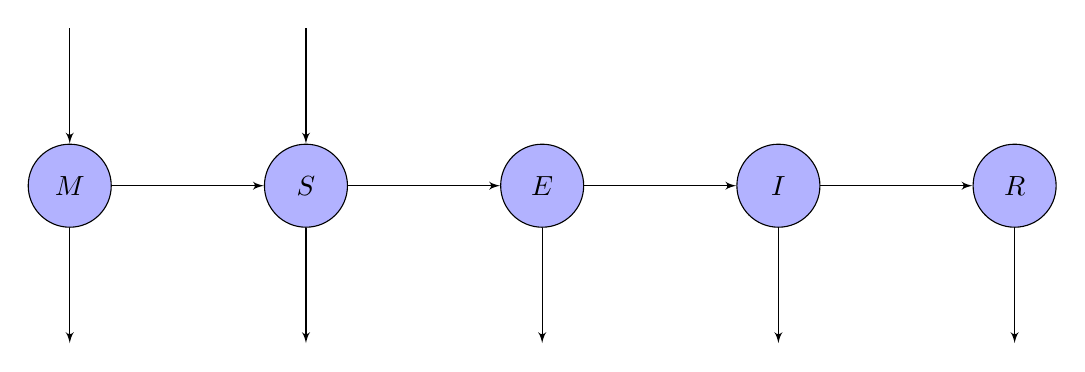
\begin{tikzpicture}[node distance=3cm,auto,>=latex',every node/.append style={align=center}]
  \node [int,  fill = white!70!blue] (s)              {$S$};
  \node[int, fill = white!70!blue] (m) [left of=s] {$M$};
  \node [int,  fill = white!70!blue] (e) [right of=s]             {$E$};
  \node [int,  fill = white!70!blue]           (i) [right of=e] {$I$};
  \node [int,  fill = white!70!blue] (r) [right of=i] {$R$};
  \path[->, auto=false] (s) edge node {} (e)
  (e) edge node {} (i)
  (i) edge node {} (r)
  (m) edge node {} (s)
  ++ (0,2) edge node {} (m)
  (s) ++ (0,2) edge node {} (s);
  \path[->]   (m) edge node {}  ++ (0,-2);
  \path[->]   (s) edge node {}  ++ (0,-2);
  \path[->]   (e) edge node {}  ++ (0,-2);
  \path[->]   (i) edge node {}  ++ (0,-2);
  \path[->]   (r) edge node {}  ++ (0,-2);
\end{tikzpicture}
\caption{Depiction of a MSEIR model with birth and death rates.  $M$ - passive immunity from mother; $S$ - susceptible; $E$- exposed, latent; $I$- infected; $R$ - recovered.  An arrow out of the system indicates death and an arrow into the system indicates birth.}\label{fig::mseir}
\end{figure}


This compartment model approach includes not only the exposed, latent compartment $E$ but additionally the compartment $M$ which stands for passive immunity inherited from the mother.  \cite{hethcote2000} describe the model with the following set of ODES that include birth rate $b$ and death rate $d$, respectively (reparametrized to match our notation),
\begin{align*}
  \frac{dM}{dt} &= b(N-X) - (\delta + d) M \\
  \frac{dX}{dt} &= bX + \delta M - \frac{\beta XY}{N} - dX\\
  \frac{dE}{dt} &= \frac{\beta XY}{N} - (\epsilon + d) E\\ 
  \frac{dY}{dt} &= \epsilon E - (\gamma + d) Y \\
  \frac{dZ}{dt} &= \gamma Y - dZ \\
  \frac{dN}{dt} &= (b-d)N,
\end{align*}
where $\delta$ is the rate of passive, immune infants transitioning to susceptible indnividuals, $\beta$ is the rate of infection, $\epsilon$ is the rate of of infectious individuals becoming infected, and $\gamma$ is the rate of recovery.  The reproduction number is then,
\begin{align}\label{eq:r0-mseir}
\rr &= \frac{ \beta \epsilon}{ (\gamma + b)(\epsilon + b)}.
\end{align}
\cite{hethcote2000} note that this calculation of $\rr$ may be strictly derived through interpretation of the definition, as ``$\rr$ is the product of the contact rate $\beta$ per unit time, the average infectious period adjusted for population growth of $\frac{1}{\gamma + b}$ and the fraction $\frac{\epsilon}{\epsilon + b}$ of exposed people surviving the latent class $E$.''  They note that this model is well suited for diseases such as measles, rubella, or mumps where the mother may pass some antibodies to her newborn.  This expression may also be derived using the next generation operator described in Section \ref{sec:ngm}.

Again, this is simply a model for transmission of a disease and does not specify how $\rr$ is to be estimated once the model is written down.  Method such as least squares and MLE are common ways to estimate the parameters in this model and hence $\rr$.  When the birth rate $b=0$, note that $\rr$ reduces to the derived expression for both the SIR and SEIR models without birth and death rates, $\frac{\beta}{\gamma}$.




\subsubsection{Amplifier Model (AMP)}
As mentioned previously, compartment models may be arbitrarily complex.  We demonstrate this idea with a set of compartments for each strain of a disease like influenza or HIV.  \cite{blower2004} discuss the case where a disease may have different strains and consequently a different reproduction number for each strain.  They introduce a multistrain mathematical model called the amplifier model to deal with this case.

This model is based on the the SEIR compartment model, accounting for a number of strains simultaneously.  There is a set of ODEs for each strain of the disease with different parameters for recovery, transmission rate, and drug resistance of the disease.  Additionally, there is mixing of the different strains as ``the amplifier model also allows for immigrating and emigration of individuals of all types, as well as reinfection of latently infected individuals'' \citep{blower2004}.  The details may be found in their manuscript.  Ultimately, their derivation for $\rr^{(i)}$ where $i$ stands for the $i$th strain is
\begin{align*}
\rr^{(i)} = X^* \frac{ ( \beta_i^Y + \beta_i^E)\nu_i + \beta_i^Y \mu_i^E}{(\nu_i + \mu_i^E)(c_i + k_{i,i+1} + \mu_i^Y)}.
\end{align*}
Here, $X^*$ is the number of susceptibles individuals in the disease-free equilibrium in the absence of immigration or emigration; $\beta_i^E$ and $\beta_i^I$ are strain-specific transmission rates for the latent, and infected classes, respectively; $\nu_i$ denotes the progression rate from latently infected to disease for strain $i$; $\mu_i^E$ and $\mu_i^{Y}$ are death rates for the latent and infected classes, respectively; $c_i$ is the cure rate; and $k_{i, i+1}$ is a parameter associated with the degree of amplification of drug resistance.  They note that ``each reproduction number is the product of average number of secondary infections caused per unit time, the aver time a case remains infectious and the probability that an infected individual develops disease.''

In the amplifier model, $\rr$ was derived from using the stability point (disease free equilibrium state in the absence of immigration or emigration) of the system by solving the characteristic polynomial for the eigenvalues.  This derivation is explained in more depth in Section \ref{sec:ngm}.

We describe this model as opposed to other available CMs because it shows not only how complicated CMs can become, but also to demonstrate how researchers approach the often controversial assumption of homogeneity.  In this case, we have strain-specific transmission rates, so we are essentially stratifying compartments into different groups, allowing for some heterogeneity.  A disadvantage is the amount of typed data required to estimate all parameters, which may be estimated through the usual methods such as least squares and maximum likelihood estimation.


\subsubsection{Next Generation Model (NGM)}
\label{sec:ngm}

Very complicated models have arisen from stratification of compartments such as one with 26 compartments \citep{pandey2014}.  As such, there is a need to be able to derive an expression for $\rr$ regardless of the structure of the compartment model.   The Next Generation Model (NGM) is a generalization of any compartment model at the infection-free steady state. This model solves the problem of having an expression of $\rr$ in terms of the epidemiological parameters for a general compartment model.  Originally, introduced by \citep{diekmann1990}, \cite{diekmann2009} posit a recipe to find $\rr$ for a wide class of compartment models, including commonly used ones such as MSEIR, MSEIRS, SEIR, SEIRS, SIR, SIRS, SEI, SEIS, SI, and SIS \citep{hethcote2000}. We summarize that recipe here, using their notation.  First, define the \textit{infected subsystem} as ``the equations of the ODE system that describe the production of new infections and changes in state among infected individuals.''  Let $x = (C_1, C_2, \dots, C_m)$ where $C_i$ are the different compartments of the infected subsystem.  The steps to find $\rr$ are as follows:


\begin{enumerate}
\item ``Linearize the infected subsystem of nonlinear ODEs about the infection-free steady state''
\item Decompose the linearized infected subsystem into $(T + \Sigma )x$ where $T$ is a $m\times m$ matrix of transmissions and $\Sigma$ is a $m \times m$ matrix of transitions.
\item $\rr$ is the spectral radius (i.e. the dominant eigenvalue) of $K_L=-T \Sigma^{-1}$.  Here $L$ stands for the ``large domain.''
\end{enumerate}

Here, $T_{ij}$ is the rate of transmission of \textit{newly} infected individuals in state $i$ created by individuals in state $j$.  $\Sigma_{ij}$ is the transition rate of individuals into compartment $i$ from compartment $j$.

This method has the assumptions of a basic compartment model: homogeneous mixing among populations and the law of mass action, i.e., that the number of infected individuals are proportional to the number of infected individuals at the previous step.  The estimations for $\rr$ from the previously mentioned compartment models may also be derived using this method.  Additionally, this method is advantageous in that the matrix $\Sigma$ and $T$ have intuitive. 

Although, this method is useful for deriving an expression of $\rr$, it is unclear how to actually estimate it from these expressions.  One could use maximum likelihood if one specifies distributions for how compartments change over time or least squares may be applied. In general, adding numerous compartments is often tedious and difficult and needlessly complicated.  Instead, researchers have started to lean towards ABMs when introducing heterogeneity in their models, which we describe in Section \ref{sec:network}.  Another disadvantage, is that $\rr$ is only derived using the disease-free steady state, which is an approximation.  

%%%%%%%%%%%%%%%%%%%%%%%%

\subsection{Exponential Growth}\label{sec:exp-growth}
Typically, CMs expressed through differential equations have no known analytical solutions, which makes deriving a closed-form expression for $\rr$ difficult or impossible.  One simplification that is often introduced to the SI-framework is that of exponential growth, or that the number of infections in the beginning of an epidemic mimics that of an exponential curve.  This simplified expression has allowed for many derivations of $\rr$.


\subsubsection{Exponential Growth (EG)}
\label{sec:expgrowth}
\cite{wallinga2007generation} report that the effective reproduction number $\mathcal{R}_t$ and hence the initial reproduction number $\rr$ may derived using the fact that infection ``counts increase exponentially in the initial phase of an epidemic.''  We then have to estimate $r$, the \textit{per capita} change in the number of new cases per unit of time and $\omega$ the serial interval. Then, we have
\begin{align}\label{eq:lotka}
\rr = \exp{(r \omega)}
\end{align}
or its first order approximation
\begin{align}\label{eq:anderson}
\rr = 1 + r \omega.
\end{align}
Equation \eqref{eq:lotka} is derived from a demographic view using the Lotka-Euler survival equations which come from the fields of demography, ecology, and evolutionary biology, whereas Equation \eqref{eq:anderson} is derived through an epidemiologist's perspective.  These estimates for $\rr$ obtained from Equation \eqref{eq:lotka} and Equation \eqref{eq:anderson} can be strikingly different in practice.

\cite{wallinga2007generation}, instead, use a moment generating function expression for $\rr$.  With $\omega(t)$ as the serial interval, then
\begin{align*}
\rr^{-1} &= \int_{a=0}^\infty e^{-rt}\omega(t)dt.
\end{align*}
For all these above estimations of $\rr$, we observe the duration of serial intervals in a period of exponential growth.  Deciding when exponential growth occurs and which data points to use to estimate $\rr$ is difficult.  \citeauthor{wallinga2007generation} specify $\omega$ in multiple ways.  Parametrically, they use exponential, normal, and delta distributions.  They also observe the empirical distribution of the serial interval.

\citeauthor{wallinga2007generation} note that specifying the epidemic model ``implicitly specifies a generation interval distribution.''  The above equations are under the SIR framework, but this method may be adapted to acommodate frameworks such as the SEIR model and more.

\subsubsection{Maximum Likelihood Estimator of Secondary Infections (MLSI)}\label{sec:mle-si}
A common method used to estimate parameters in the SI-framework is maximum likelihood estimation.  This method requires knowing the likelihood of a parameter given the data observed, and hence many distributions may be specified.  The MLE of secondary infections, described by \cite{forsberg2008}, finds the estimate of $\rr$ by maximizing the likelihood function under a certain assumptions.  We assume that the ``the number of secondary cases produced by an infected individual follows a Poisson distribution, and that the serial interval is described by a multinomial distribution.''  Recall, the serial interval is the distribution of time between a primary case developing symptoms and a case infected by the primary case developing symptoms.  An approximate version of this can be simplified to a thinned Poisson in Equation \ref{eq:mlesi} where
\begin{align}\label{eq:mlesi}
  L(\rr, \mathbf{p}) = \prod_{t=1}^T \frac{e^{- \rr \sum_{j=1}^{\min(k,t)}J_{t-j}p_j}\left (\rr \sum_{j=1}^{\min(k,t)}J_{t-j}p_j \right )^{J_t}}{J_t!}.
\end{align}
Here, $k$ is the maximal amount of the serial number, $T$ is the total time and $p_j$ is the probability of displaying symptoms on day $j$ after being infected.  The number of cases on day $t$, $J_t$ are incidence counts that are known. 

This method assumes a Poisson distribution on $\rr$ in addition to assuming a multinomial on the serial interval.  Additionally, this method also assumes a period of exponential growth.  An advantage is that assuming a Poisson distribution has nice properties which make it possible derive some of the statistical properties of this method.  Two disadvantages are that we only have an approximation for $\rr$ and have to decide which data points to use in a certain time frame.  Additionally, we hae to validate our assumptions about the specified distributions.


%%%%%%%%%%%%% 5

\subsubsection{Time Dependent Reproduction Number (TDR)}\label{sec:timedep}
Another likelihood based approach to estimate $\rr$ is that of the time dependent reproduction number, as described by \cite{forsberg2008}.  Here, we maximize the likelihood that case $i$ has been infected by case $j$ at certain time using the serial interval, $w(t)$ where $t_i$ is when case $i$ was infected and $N$ is the total number of cases,
\begin{align*}
  p_{ij} &= w(t_i- t_j) / \sum_{i \neq k} w(t_i - t_k),\\
  \rr &= \frac{1}{Y(0)}\sum_{i=1}^N p_{i0}
  \end{align*}
  A disadvantage of this method is that it assumed we have some idea about the generation interval distribution, $w(t)$, but an advantage is that there is no explicit assumption on the distribution of $\omega$.  This method also requires that the initial number of susceptibles $X(0)$ is roughly the size of the total population.  Another advantage is the explicit use of distributions to indicate that $\rr$ is indeed a random variable.

\subsubsection{Initial Growth Rate and Final Size (IGRFS)}
\label{sec:igr-fs}

Initial growth rate, as described by \cite{dietz1993estimation} is derived by \cite{anderson1986}, initially to study the spread of HIV estimates $\rr$ through
\begin{align*}
\rr = \frac{D \ln 2} {t_d} + 1,
  \end{align*}
  with $D$ as the average incubation period and $t_d$ as the doubling time during its early stages.  This method assumes one knows when the ``early stage'' ends along with knowledge of the average incubation period.  

  Final size, on the other hand, only looks at $\rr$ once a disease has run its course.  Here $\mu_0$ is the proportion of initially infected individuals and $\mu_\infty$ is the final, cumulative proportion of infected cases at the end of an epidemic,
\begin{align}\label{r0_attackrate}
\rr =  \frac{\log \left (\frac{1  - \mu_0}{X(0)/N}  \right ) }{\mu_0 - (1 - X(0)/N)}
\end{align}
This method can only be used to assess $\rr$ after a disease has passed through a population.  Additionally, if either $\beta$ or $\gamma$ were affected during the disease's lifetime, such as through interventions and prevention strategies, then $\rr$ cannot be properly assessed.

  These two methods allow one to look at $\rr$ at both the beginning and the end of an epidemic.  However, both approaches have advantages and disadvantages.  For the initial growth rate, while one can see $\rr$ at early stages, estimating the doubling time $t_d$ is difficult.  For final size, one has to wait until the end of an epidemic to calculate $\rr$, and preventions of the disease may skew the final result.
%%%%%%%%%%%%%%%%%%%%%%%%%%%%%%

  \subsection{Estimation from Networks}
As estimating $\rr$ is concerned with the number of new infections based on the contacts of old infections, a network is a seemingly intuitive way to model such contacts and hence infections.  Networks that have been used to estimate $\rr$ include contact tracing of actual individuals, branching processes to model the spread of disease, and agent-based models (also known as individual level models), which all leverage networks along with different sources of data to generate estimates of $\rr$.  Additionally, networks provide an intuitive framework in which individuals can interact with varying levels of heterogeneity.
  
\label{sec:network}

%%%%%%%% 5
\subsubsection{Contact Tracing (CT)}
\label{sec:contact_tracing}
A reasonable idea to estimate $\rr$ is to directly observe the number of secondary infections produced by an initial infector.  However, this approach is generally impractical as it is difficult to estimate every single contact an individual may have.   With seriological information, we could conceivably recreate the transmission of the disease throughout a population.  Even in this case it is unlikely, for one, to have a completely susceptible population, which is essential to an unbiased estimate of $\rr$.  Moreover, this would implicitly be conditioning on the initial infector's contacts which may not reflect those of the rest of the population.  We write the calculation for $\rr$ under contact tracing in Equation \ref{eq:r0_contacttracing}, where $X_0$ is a random variable denoting the number of individuals in the population individual 0 infects.  Here $S_0=N$ indicates that the initial number of susceptibles is $N$, the size of the population,
\begin{align}\label{eq:r0_contacttracing}
\rr = E[ X_0 | S_0 = N].
\end{align}
\cite{eames2003} describe contact tracing as an ``extreme form of targeted control, where the potential next-generation cases are the primary focus,'' that is, one focuses on treating the contacts of an infected individual rather than applying uniform treatment across a population.  They note that this method has ``proved to be a highly successful strategy when the number of infectious cases is low'' and ``is the standard tool for eliminating minor outbreaks in the latter stages of disease eradication.''

They describe an estimate for $\rr$ for a SIR model on a network, with $r$ as the rate of transmission across a contact multiplied by the infectious period and $n$ as the number of contacts as
\begin{align*}
\rr = r(n-2)
\end{align*}
Again, the difficulties of this method lies in one, estimating the contacts of an initial infected individual and two, extrapolating the contacts of the initial individual to the population as a whole.  As such, although vital in treating a disease in its early stages, is not the best choice to estimate $\rr$ due to the high level of uncertainty inherit in the method.


%%%%%%%%%%%%%%%%%%%%%%%%%%%%%%%%

\subsubsection{Branching Process (BP)}
\label{sec:branching-process}

Branching processes are models for population growth which track generations of new offspring.  We describe branching processes as adapted for epidemic modelling from the notation of \cite{grimmett1992}.  An infector $i$ may produce new infections, called offspring, over the duration of the  infector $i$'s disease.  The offspring of the original infector directly produces are called the first generation.  The offspring of the first generation are called the second generation and so on.  An important assumption in branching processes is that the offspring produced from different infectors are indepedent and identically distributed, and so for a branching process to be a valid model in epidemic modeling, we must assume a large population with few infectors.

\com{draw a family tree}

\cite{getz2006} give a way to calculate $\rr$ from a branching process.  ``We define the offspring distribution $\{q_i \}_{i=0}^\infty$, where $q_i$  is the probability that an infectious individual infects $i$ other individuals.  Thus we require $\sum_{i=0}^\infty q_i =1$ and note that $\rr$, the mean number of cases contracting disease from each infective'', is simply given by'
  \begin{align*}
    \rr = \sum_{i=0}^\infty iq_i.
  \end{align*}
  It is assumed we know how to estimate the $q_i$, and so in this case, it is not too different of an approach than contact tracing.  The disadvantages of this method are similar to that of contact tracing as data about which individuals  infected another is very difficult to obtain.  An advantage is that this method directly gets to the ``heart'' of the definition of $\rr$ as it is concerned with generations of infected individuals rather than incidence at a certain time.


    

\subsubsection{Agent-Based Models (ABM)}
\label{sec:agent-based-models}
Agent-based models (ABMs) or individual level models (ILMs) are ``bottom-up'' models, meaning micro patterns are simulated and macro patterns are then inferred from these micro patterns.  ABMs consist of agents which represent individuals (e.g., people, mosquitoes, poultry) and a series of activities in which the agents can affect one another and evolve over time.

In epidemiology, ABMs may be used to simulate the spread of disease.  ABMs allow for every detail of an infection to be known, in the context of estimating $\rr$, meaning we know exactly who is infected by whom and when.  Thus $\rr$ can be estimated simply through
\begin{align*}
  \rr = \frac{1}{\# \text{ simulations}}\frac{1}{\#\text{ initial infections}} \sum_{(s \in \text{ simulations})}\sum_{(i \text{ infected at } t=0)} \# \text{ infected by $i$ in simulation }s.
\end{align*}
Examples of estimations of $\rr$ using ABMs/ILMs are in \cite{breban2007,ahmed2013variance}.

There are many advantages to using ABMs, a main one being able to run the model multiple times under the same initial conditions.  In this way, one can easily obtain variance estimates of $\rr$ in addition to empirical distributions of it.  Moreover, this estimation can accommodate any model specification of how the disease is transmitted through the population.  However, the major disadvantage of the ABM lies in calibrating the evolving of agents over time to accurately reflect reality, a problem that cannot be understated.  Thus, it is typically necessary to have knowledge of parameters such as the serial interval, transmission rate, recovery rate, etc.  Additionally, we need to have accurate agents in number, characteristics, and their implied network structure.  ABMs are flexible in that they may be used with any model in the SI framework.  The only requirement is that we track who infects whom and can adapt for any additional states such as exposure or prevention strategies such as closing schools \citep{fred}.







\subsection{Variance Methods}
\label{sec:methods}

Estimating $\rr$ is difficult and estimating $V[\rr]$, the variance, is even moreso.  We describe general methods which may be applicable to estimate the variance.  We describe the assumptions that are used along with each method and note that they may not be applicable to all of our methods.  Still, reporting confidence intervals, or at the very least, standard deviations is very important and we hope to encourage this practice by describing the below methods used to estimate models in the SIR framework in a simple fashion.  Regardless of the method used to estimate variance, confidence intervals, or credible intervals, we encourage researchers to carefully examine all underlying assumptions of 1) specifying a model for disease transmission, 2) estimating $\rr$ from the model, and 3) the method used to estimate the variance or CIs.


\subsubsection{Delta Method}\label{delta-method}

When the method estimates \(\beta\) and \(\gamma\) instead of \(\rr\) directly, we use the delta method approximation to calculate the
variance of \(\rr\). Here, we know \(\rr = h(\beta, \gamma) = \frac{\beta}{\gamma}\). Then \(\bigtriangleup h = (\frac{1}{\gamma},  -\frac{\beta}{\gamma^2})^T\).  Then \(V[\rr] = \bigtriangleup h^T \Sigma_{\beta, \gamma} \bigtriangleup h\), where \(\Sigma_{\beta, \gamma}\) is covariance matrix of \(\beta\) and \(\gamma\).

This estimate assumes that the distribution of $\beta$ and $\gamma$ are asymptotically normal.  Here, we use the relationship of $\rr = \frac{\beta}{\gamma}$ in order to estimate the variance, which is specific to the SIR framework.  This method may be extended to other frameworks and we provide some examples here \com{add examples of SEIR, serial interval, etc.}.  The advantages of the delta method are that as the NGM posits a recipe to derive $\rr$, then it is theoretically possible to use the delta method to derive an expression for an expression of variance for any compartment model.

\subsubsection{Sensitivity Analysis}\label{sensitivity-analysis}

Sensitivity analysis is used to measure how robust estimates are to change.  If small changes in our estimated parameters do not change our estimates for the number of infected by much, then we may prefer this method to another.  For the SIR model, we estimate \(\frac{\partial Y}{\partial \beta}\) (or \(\frac{\partial Y}{\partial \rr}\) when using reparametrized least squares) and \(\frac{\partial Y}{\partial \gamma}\) at each time point \(t\) using the estimated \(\beta\) or \(\gamma\) from the estimation process where $Y(t)$ stands for the number of infected at time $t$.  More generally,  let $Y(t_i) = f(t_i, \theta)$ where $\theta$ is a vector of parameters. Then an approximation of the covariance matrix is \((\chi^T \chi)^{-1}\) where \(\chi_{ij} = \frac{ \partial Y(t_i)}{ \partial \theta_j}\). \com{add citation}.  Advantages of this method include that it is a standard way to estimate the variance of $\rr$.

\subsubsection{Posterior Distribution}
When one uses a Bayesian approach to estimate $\rr$, the result should be a distribution rather than an estimate.  One can simply look at the quantities of this distribution to form a credible interval for this estimate.  Advantages of this method include having an entire distribution compared to a point estimate.  One disadvantage is that the Bayesian approach will not guarantee frequentist properties that epidemiologists may be looking for such as being able to compare diseases to one another.



%%%%%%%%%%%%%%%




\section{Analysis and Results}
\label{sec:results}

\section{Discussion}
\label{sec:dis}


\label{sec:details}




\bibliographystyle{apa}%Choose a bibliograhpic style
\bibliography{Master}


\appendix

\section{Epidemic Modeling Terminology}
\label{sec:term}

Here we summarize some of the terminology and notation used throughout the methods for estimating \rr.

{$\rr$} -- reproduction number -- 

{$\mathcal{R}_t$} -- effective reproduction number

{$\beta$} -- the infection rate

{$\gamma$} -- inverse of the expected recovery time

{$N_t$} -- Number of individuals in the population at time $t$

{$X(t)$} -- the number of susceptible individuals in a population at time $t$

{$Y(t)$} -- the number of infected individuals in a population at time $t$

{$Z(t)$} -- the number of recovered individuals in a population at time $t$

{$\omega$} -- serial or generation interval -- the time from onset of symptoms in an index case to the onset of symptoms in a subsequent case infected by the index patient

AR -- attack rate -- percentage of the population eventually infected




\end{document}


%%%%%%%%%%%%%%%%%%%%%%
\Textbf{Title:} 

\textbf{Author:} 

\textbf{Citation:} 

\textbf{Major themes:} 

\textbf{Notes:}
\\
%%%%%%%%%%%%%%%%%%%%%%




\begin{figure}[h]
\begin{center}
\includegraphics[width=4in]{mvhw7_3c.pdf}
\end{center}
\caption{
Biplots of the different continuous variables and their correlations.}\label{fig3c}
\end{figure}

%% two pictures whoa

\begin{figure}[h]
\centering


\begin{figure}[h]
\centering

\begin{subfigure}{.5\textwidth}
  \centering
  \includegraphics[width=1\linewidth]{mt_eda_cont_hists.pdf}
  \caption{Histograms of Arrival Delay and continuous covariates.  Arrival delay seems to have a right skewed distribution.  This may indicate that we will be transforming this variable later on.  After transforming Air Time and Distance by a log transformation, we don't really seem to have many outliers in our covariates.  We seem to have outliers in the CRS Dep. Time and Arrival Time; however, time is cyclical and so these are not, in fact outliers.}
  \label{hists}
\end{subfigure}%
\begin{subfigure}{.5\textwidth}
  \centering
  \includegraphics[width=1\linewidth]{mt_eda_cont_hists.pdf}
  \caption{\textcolor{red}{Placeholder}}
  \label{tabs1}
\end{subfigure}
\caption{}
\end{figure}







%%
\begin{figure}
\centering
\begin{subfigure}{.5\textwidth}
  \centering
  \includegraphics[width=1\linewidth]{resids_full.pdf}
  \caption{}
  \label{residsf}
\end{subfigure}%
\begin{subfigure}{.5\textwidth}
  \centering
  \includegraphics[width=1\linewidth]{diags_full.pdf}
  \caption{ }
  \label{diagsf}
\end{subfigure}
\caption{}
\end{figure}




